\documentclass[10pt,a4paper]{minimal}
\usepackage{pgfplots}

\pgfplotsset{
	integral segments/.code={\pgfmathsetmacro\integralsegments{#1}},
	integral segments=3,
	integral/.style args={#1:#2}{
		ybar interval,
		domain=#1+((#2-#1)/\integralsegments)/2:#2+((#2-#1)/\integralsegments)/2,
		samples=\integralsegments+1,
		x filter/.code=\pgfmathparse{\pgfmathresult-((#2-#1)/\integralsegments)/2}
	}
}

\begin{document}
	
	%\pagecolor{black}
	
	\begin{center}
		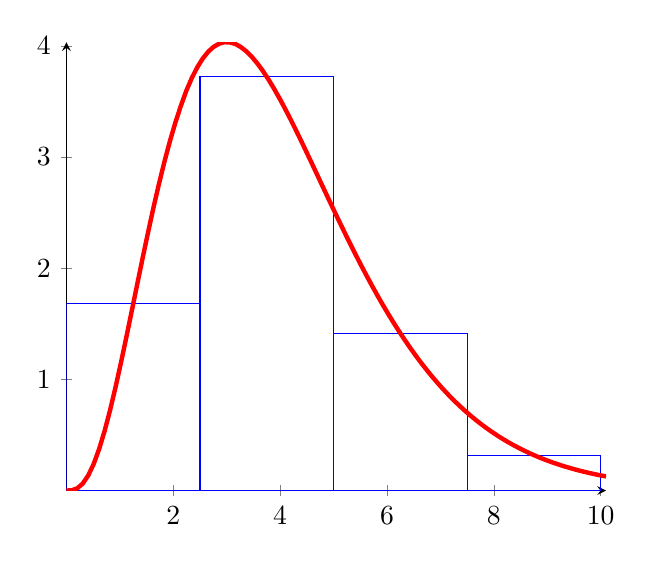
\begin{tikzpicture}[color=black,/pgf/declare function={f=3*e^(-x)*x^3;}]
			\begin{axis}[
				domain=0:10.1,
				samples=100,
				axis lines=middle
				]
				\addplot [
				blue,
				integral segments=4,
				integral=0:10
				] {f};
				\addplot [ultra thick,color=red] {f};
				
			\end{axis}
		\end{tikzpicture}
	\end{center}
	
\end{document}